\documentclass[10pt,ignorenonframetext,]{beamer}
\setbeamertemplate{caption}[numbered]
\setbeamertemplate{caption label separator}{: }
\setbeamercolor{caption name}{fg=normal text.fg}
\beamertemplatenavigationsymbolsempty
\usepackage{lmodern}
\usepackage{amssymb,amsmath}
\usepackage{ifxetex,ifluatex}
\usepackage{fixltx2e} % provides \textsubscript
\ifnum 0\ifxetex 1\fi\ifluatex 1\fi=0 % if pdftex
  \usepackage[T1]{fontenc}
  \usepackage[utf8]{inputenc}
\else % if luatex or xelatex
  \ifxetex
    \usepackage{mathspec}
  \else
    \usepackage{fontspec}
  \fi
  \defaultfontfeatures{Ligatures=TeX,Scale=MatchLowercase}
\fi
\usetheme[]{JuanLesPins}
\usecolortheme{lily}
\usefonttheme{structurebold}
% use upquote if available, for straight quotes in verbatim environments
\IfFileExists{upquote.sty}{\usepackage{upquote}}{}
% use microtype if available
\IfFileExists{microtype.sty}{%
\usepackage{microtype}
\UseMicrotypeSet[protrusion]{basicmath} % disable protrusion for tt fonts
}{}
\newif\ifbibliography
\hypersetup{
            pdftitle={Estimaciones de Mortalidad por departamentos: el caso de la región Pampeana (2009-2011)},
            pdfborder={0 0 0},
            breaklinks=true}
\urlstyle{same}  % don't use monospace font for urls

% Prevent slide breaks in the middle of a paragraph:
\widowpenalties 1 10000
\raggedbottom

\AtBeginPart{
  \let\insertpartnumber\relax
  \let\partname\relax
  \frame{\partpage}
}
\AtBeginSection{
  \ifbibliography
  \else
    \let\insertsectionnumber\relax
    \let\sectionname\relax
    \frame{\sectionpage}
  \fi
}
\AtBeginSubsection{
  \let\insertsubsectionnumber\relax
  \let\subsectionname\relax
  \frame{\subsectionpage}
}

\setlength{\parindent}{0pt}
\setlength{\parskip}{6pt plus 2pt minus 1pt}
\setlength{\emergencystretch}{3em}  % prevent overfull lines
\providecommand{\tightlist}{%
  \setlength{\itemsep}{0pt}\setlength{\parskip}{0pt}}
\setcounter{secnumdepth}{0}

\title{Estimaciones de Mortalidad por departamentos: \newline el caso de la
región Pampeana (2009-2011)}
\author{Nicolás Sacco \footnote<.->{Penn State}; Iván Williams \footnote<.->{Universidad
  Nacional de Luján}; Bernardo L. Queiroz \footnote<.->{Cedeplar-UFMG}}
\institute{XV Jornadas Argentinas de Estudios de Población -- II Congreso
Internacional de Población del Cono Sur}
\date{Septiembre 2019}

\begin{document}
\frame{\titlepage}

\section{Introducción}\label{introduccion}

\begin{frame}{Pregunta}

\begin{itemize}[<+->]
\tightlist
\item
  Insumos para políticas de salud provinciales. ¿Qué esconden los
  \textbf{promedios provinciales}?
\item
  Escasos estudios de mortalidad en áreas menores
\item
  ``Esta en nuestros genes''
\item
  Fenómenos con un \textbf{pequeño} número de \textbf{experimentos} (y
  \textbf{desconocida cobertura})
\end{itemize}

\end{frame}

\begin{frame}{Objetivos}

\begin{itemize}[<+->]
\tightlist
\item
  Estimar la mortalidad de departamentos de la región Pampeana durante
  el período 2009-2011.
\item
  Obtener conclusiones sobre la heterogeneidad al interior de las
  provincias.
\end{itemize}

\end{frame}

\section{Datos}\label{datos}

\begin{frame}{Defunciones}

\begin{itemize}[<+->]
\tightlist
\item
  Microdatos de defunción para los años de registro 2009, 2010 y 2011 al
  Departamento de Estadísticas e Información de Salud (DEIS).\\
\item
  \emph{Residencia} y \emph{ocurrencia}.
\end{itemize}

\end{frame}

\begin{frame}

Departamento de residencia desconocido por provincia:

\begin{table}[t]

\caption{\label{tab:SinDEP}}
\centering
\begin{tabular}{l|l|r}
\hline
  & Provincia & Desc \%\\
\hline
1 & Ciudad Autónoma de Buenos Aires & 8.6\\
\hline
10 & Jujuy & 3.1\\
\hline
24 & Tierra del Fuego, Antártida e Islas del Atlántico Sur & 2.5\\
\hline
20 & Santa Cruz & 2.4\\
\hline
16 & Río Negro & 1.7\\
\hline
23 & Tucumán & 1.7\\
\hline
11 & La Pampa & 1.6\\
\hline
7 & Chubut & 1.5\\
\hline
19 & San Luis & 1.4\\
\hline
22 & Santiago del Estero & 1.2\\
\hline
\multicolumn{3}{l}{\textsuperscript{a} Fuente: en base en DEIS}\\
\end{tabular}
\end{table}

\end{frame}

\begin{frame}

Sexo Desconocido según provincia:

\begin{table}[t]

\caption{\label{tab:UnkSexAge}}
\centering
\begin{tabular}{l|r}
\hline
Dpto\_Nombre & PorcSexo\\
\hline
General Pueyrredón & 7.3\\
\hline
Vicente López & 5.6\\
\hline
Quilmes & 3.8\\
\hline
Coronel Dorrego & 3.7\\
\hline
Ituzaingó & 3.1\\
\hline
San Andrés de Giles & 2.5\\
\hline
Bahía Blanca & 2.4\\
\hline
General San Martín & 2.3\\
\hline
San Miguel & 2.2\\
\hline
La Plata & 2.1\\
\hline
\multicolumn{2}{l}{\textsuperscript{a} Fuente: en base en DEIS}\\
\end{tabular}
\end{table}

\end{frame}

\begin{frame}{Expuestos}

\begin{itemize}[<+->]
\tightlist
\item
  Población \emph{base} INDEC a 2010 + estructura observada en el censo
  2010 (INDEC, 2015)\\
\item
  Ajuste años-persona (Gonzaga \& Schmertman, 2016). Casos
  seleccionados:
\end{itemize}

\begin{figure}

{\centering 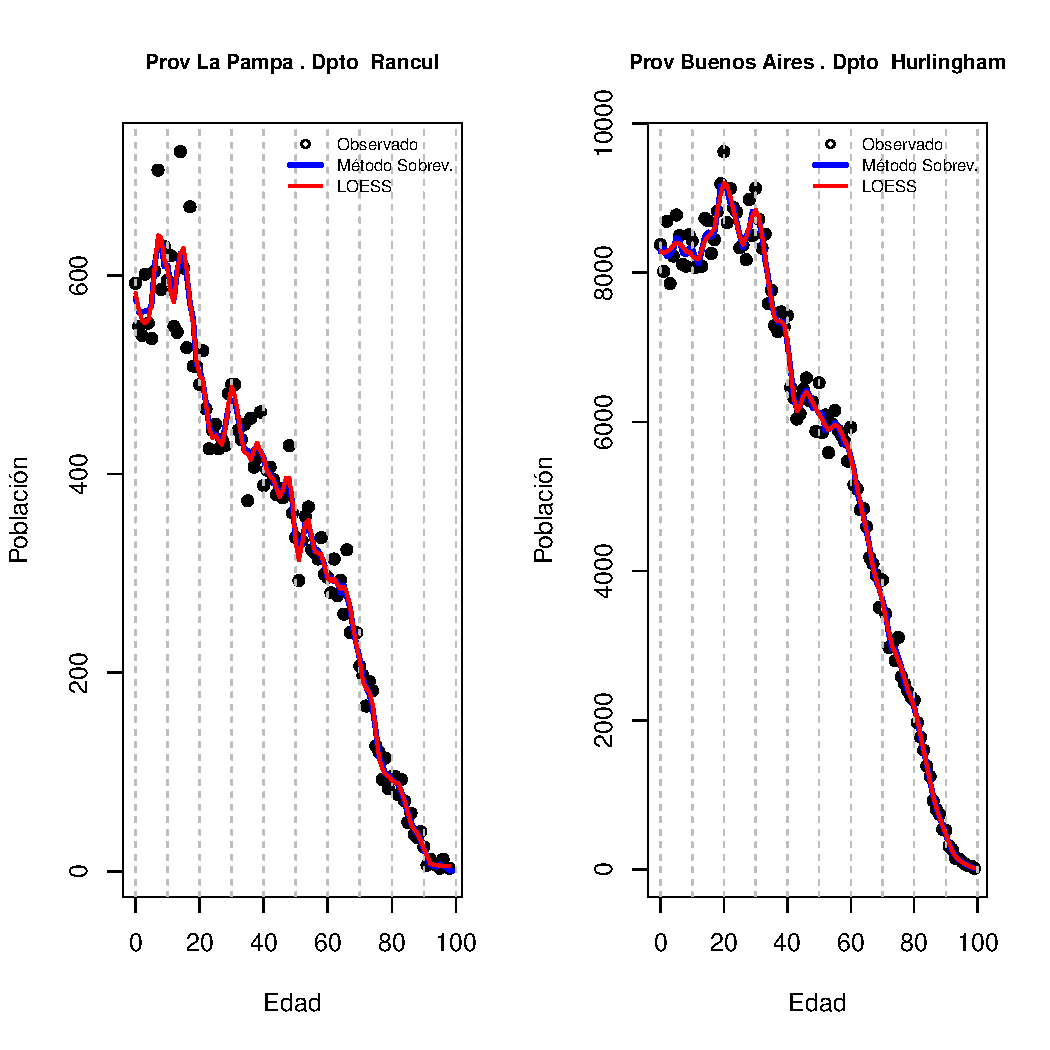
\includegraphics[width=0.5\linewidth]{C:/Proyectos/mortalidad_Argentina/analysis/plots/AdjExp2} 

}

\end{figure}

\end{frame}

\begin{frame}{Ejercicios de consistencia (1)}

\begin{itemize}[<+->]
\tightlist
\item
  Mortalidad infantil

  \begin{itemize}[<+->]
  \tightlist
  \item
    Estimación indirecta (Brass \& Coale, 1968) y tasa observada
  \end{itemize}
\end{itemize}

\pause

\begin{figure}

{\centering 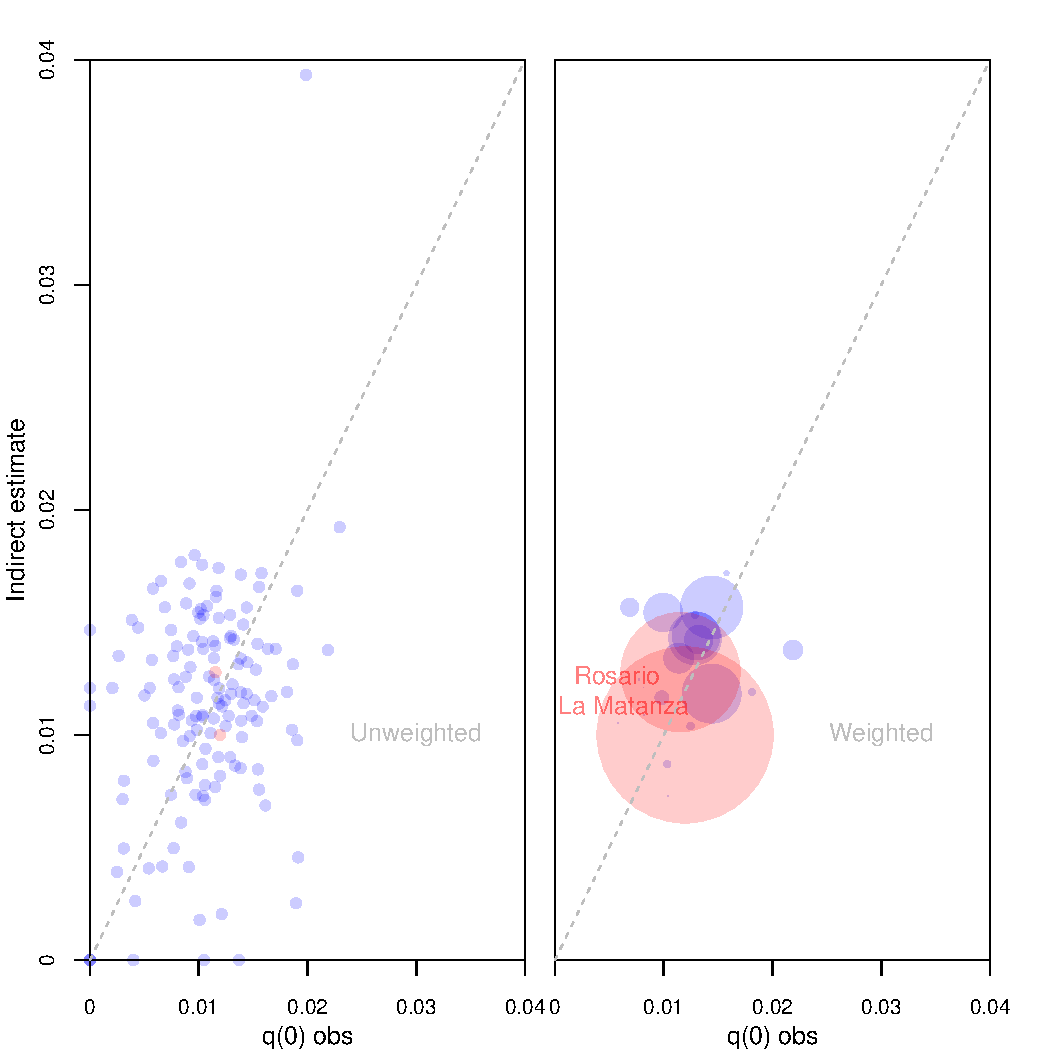
\includegraphics[width=0.55\linewidth]{C:/Proyectos/mortalidad_Argentina/analysis/plots/ChekPF} 

}

\end{figure}

\end{frame}

\begin{frame}{Ejercicios de consistencia (2)}

\begin{itemize}[<+->]
\tightlist
\item
  Relación socioeconómica \textbf{esperada}

  \begin{itemize}[<+->]
  \tightlist
  \item
    Preston (10975); Grushka et. al (2013)
  \item
    Tasa Estandarizada de Mortalidad e indicadores censales de NBI

    \begin{itemize}[<+->]
    \tightlist
    \item
      La Matanza con comportamiento ``sospechoso''
    \end{itemize}
  \end{itemize}
\end{itemize}

\pause

\begin{figure}

{\centering 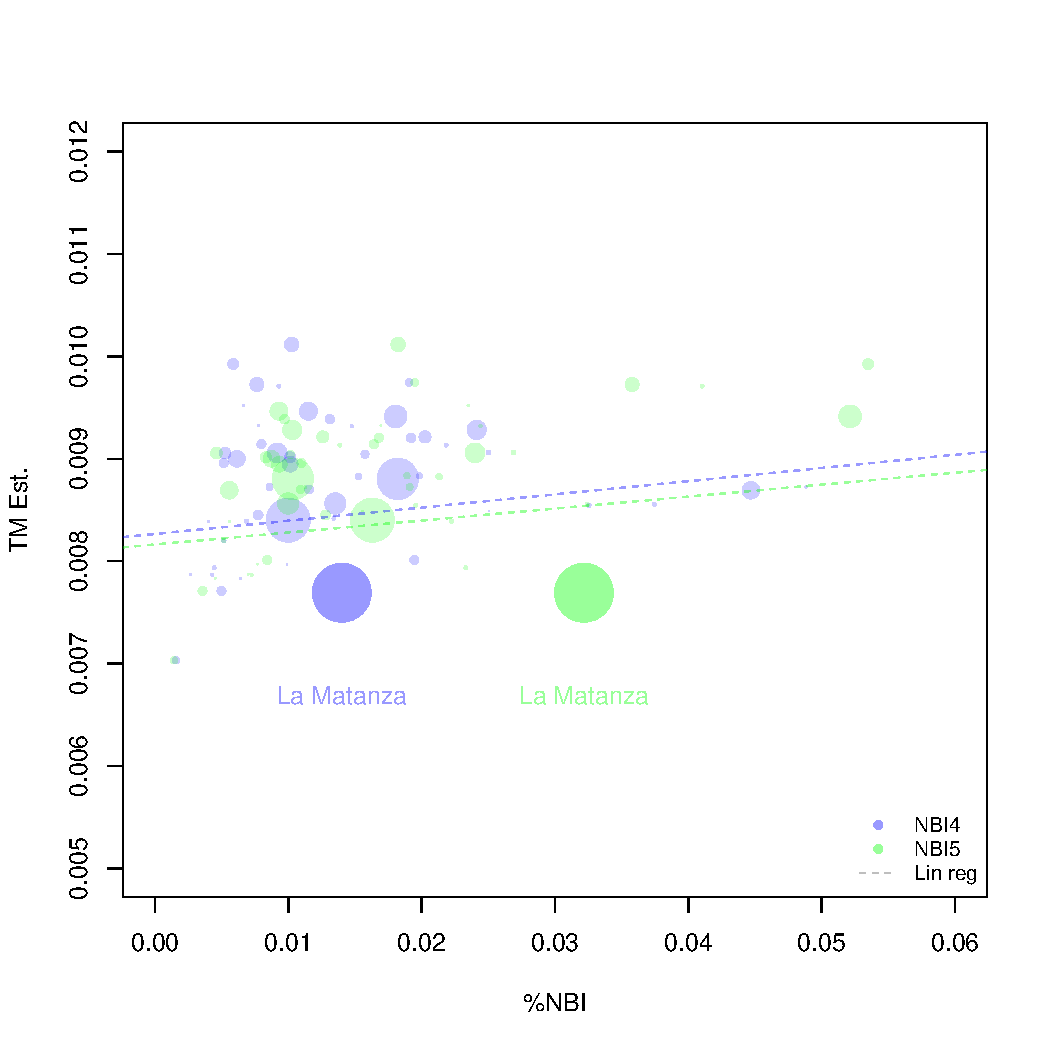
\includegraphics[width=0.6\linewidth]{C:/Proyectos/mortalidad_Argentina/analysis/plots/ChekNBI} 

}

\end{figure}

\end{frame}

\section{Metodología}\label{metodologia}

\begin{frame}

\begin{itemize}[<+->]
\tightlist
\item
  Antecedentes: Lima, Queiroz, \& Sawyer (2014); Gonzaga \& Schmertmann
  (2016); Alexander et. al (2016)
\item
  Aplicación de tres metodologías. ¿Cómo área mayor \textbf{presta}
  comportamiento?
\item
  Procedimiento:

  \begin{itemize}[<+->]
  \tightlist
  \item
    Definición de Áreas Mayores\\
  \item
    Selección metodológica de suavizamiento\\
  \item
    Construcción de tablas de mortalidad
  \end{itemize}
\end{itemize}

\end{frame}

\begin{frame}{Áreas Mayores}

\begin{itemize}[<+->]
\tightlist
\item
  Explotar similitud interna entre áreas pequeñas para poder suponer que
  su mortalidad es la realización de un proceso estocástico mayor.
\item
  Regionalización a partir de NBI estandarizado por edad.
\item
  Disminuir varianza ``intra'', aumentar varianza ``entre'' (Assuncao,
  2006)
\end{itemize}

\pause

\begin{figure}

{\centering 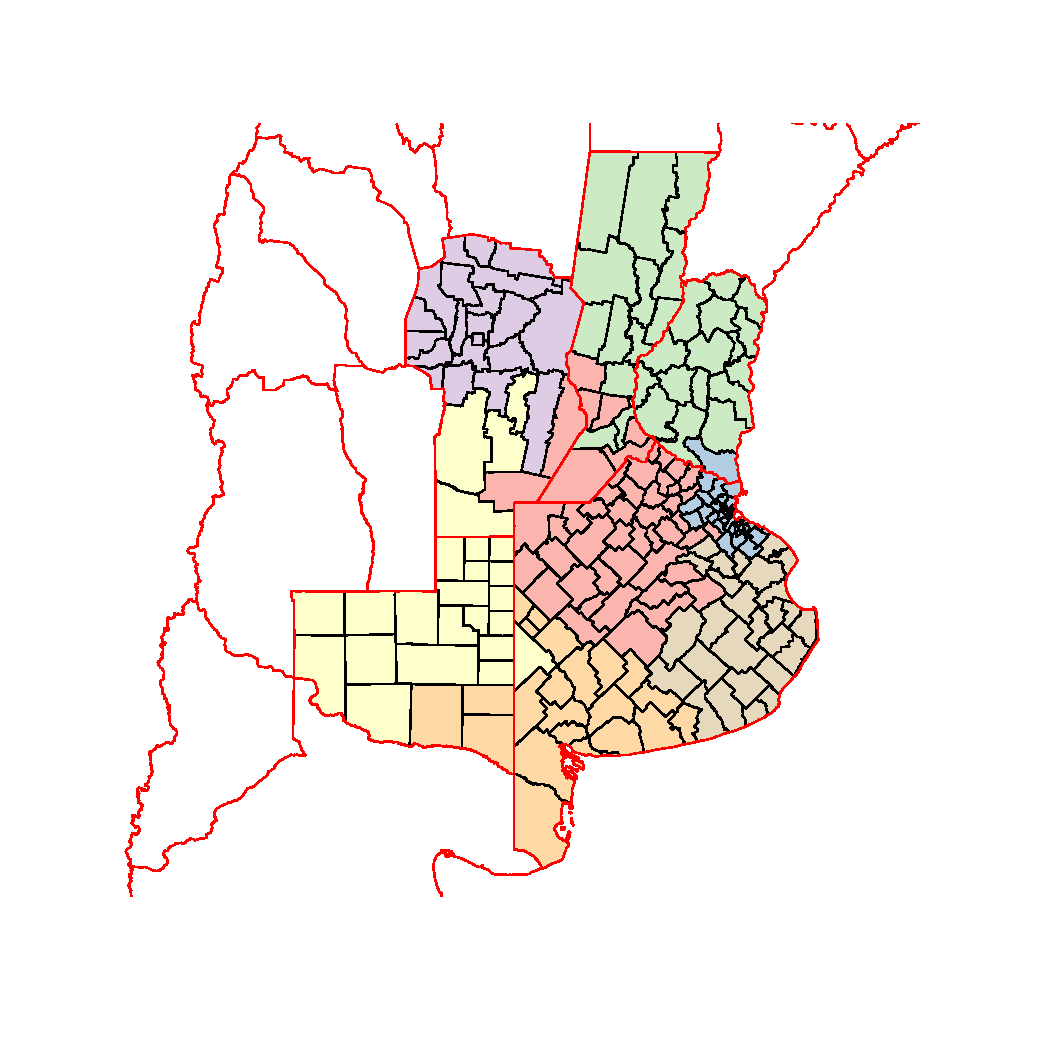
\includegraphics[width=0.6\linewidth]{C:/Proyectos/mortalidad_Argentina/analysis/plots/cluster} 

}

\end{figure}

\end{frame}

\begin{frame}{Métodos de estimación}

Se aplicaron tres métodos:

\begin{itemize}[<+->]
\tightlist
\item
  Bayes Empírico (Assuncao et. al, 2005)\\
  - La distribución a priori de cada \(m_{x,5}\) es la del área mayor\\
  - Función lineal entre \emph{observado} y \emph{a priori}, según peso
  de la varianza local respecto a la total. ``En extrema homogeneidad,
  un área menor muy pequeña podría caracterizarse a partir de la
  estimación del área más grande''"\\
\item
  TOPALS regression (Gonzaga \& Schmertmann, 2016)\\
  - Modelo Relacional. Patrón standard\\
  - Regresión spline a partir de edades ``nodos''\\
\item
  Estimación indirecta - Desplazar ``verticalmente'' estructura de
  mortalidad por edad para replicar defunciones observadas del
  departamento
\end{itemize}

\end{frame}

\section{Resultados}\label{resultados}

\begin{frame}{Ajuste}

Bayes Empírico incorpora \emph{siempre} información de departamentos muy
pequeños:

\begin{figure}

{\centering 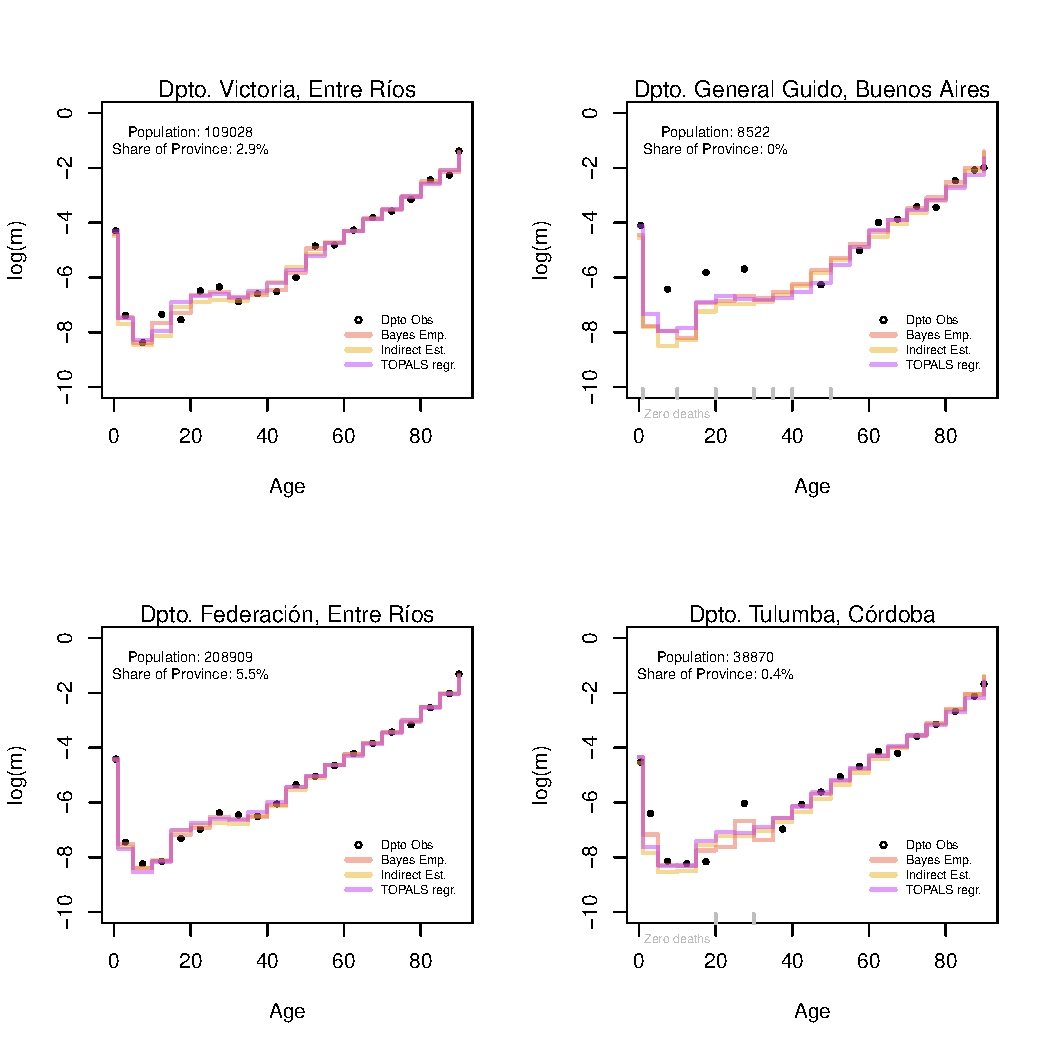
\includegraphics[width=0.7\linewidth]{C:/Proyectos/mortalidad_Argentina/analysis/plots/Ajuste} 

}

\end{figure}

\end{frame}

\begin{frame}{Análisis comparativo}

Alta correalción entre TOPALS y estimación indirecta (0.97), pero menor
en Bayes Empírico contra las demás 0.84 y 0.88.

\begin{figure}

{\centering 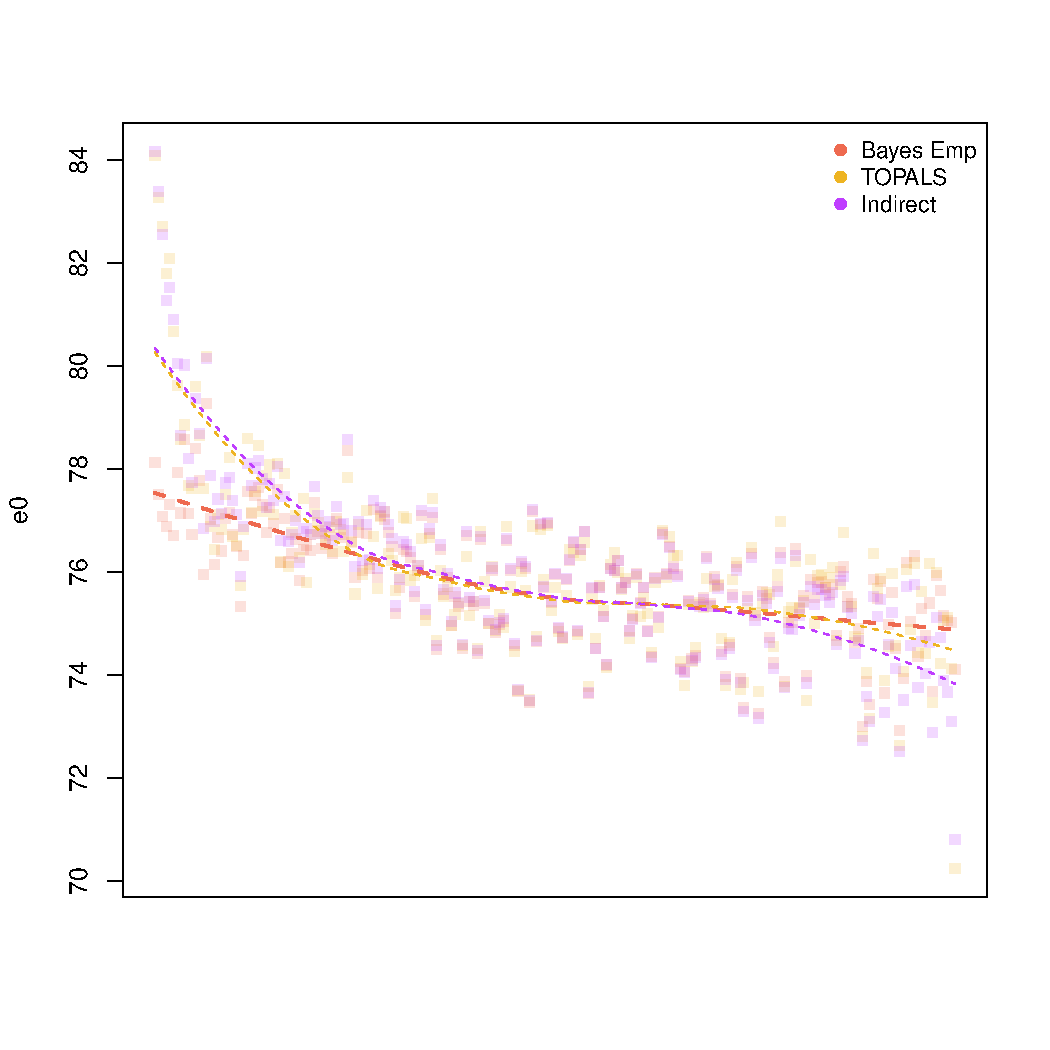
\includegraphics[width=0.7\linewidth]{C:/Proyectos/mortalidad_Argentina/analysis/plots/CompMethods} 

}

\end{figure}

\end{frame}

\begin{frame}

Casos de mayor diferencia entre métodos:

\begin{figure}

{\centering 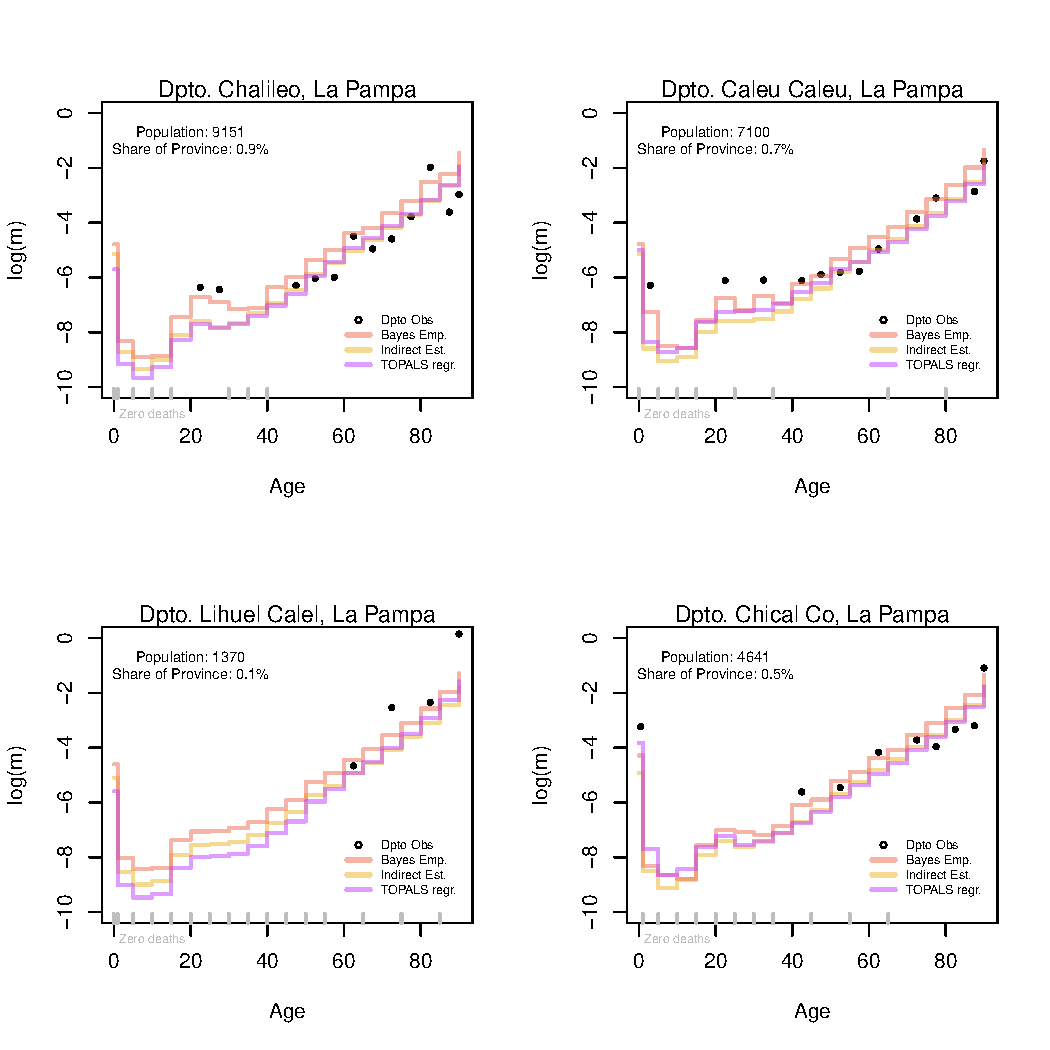
\includegraphics[width=0.7\linewidth]{C:/Proyectos/mortalidad_Argentina/analysis/plots/AjusteFeos} 

}

\end{figure}

\end{frame}

\begin{frame}{Resultados principales}

\(e_0\) según departamento: intervalos de confianza al 95\% (bootstrap):

\pause

\begin{figure}

{\centering 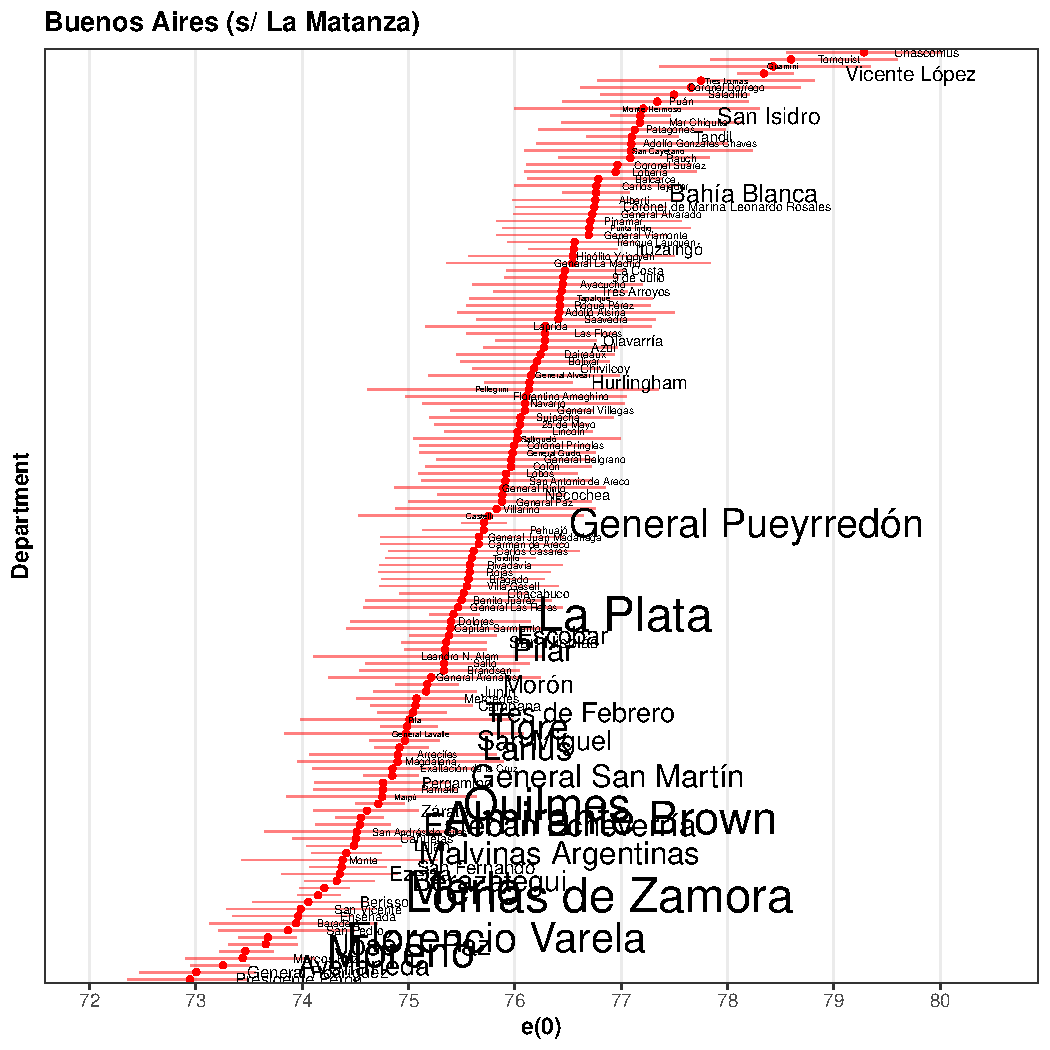
\includegraphics[width=0.6\linewidth]{C:/Proyectos/mortalidad_Argentina/analysis/plots/Buenos_Aires} 

}

\end{figure}

\end{frame}

\begin{frame}

\begin{figure}

{\centering \includegraphics[width=0.6\linewidth]{C:/Proyectos/mortalidad_Argentina/analysis/plots/Córdoba} 

}

\end{figure}

\end{frame}

\begin{frame}

\begin{figure}

{\centering \includegraphics[width=0.6\linewidth]{C:/Proyectos/mortalidad_Argentina/analysis/plots/Entre_Ríos} 

}

\end{figure}

\end{frame}

\begin{frame}

\begin{figure}

{\centering 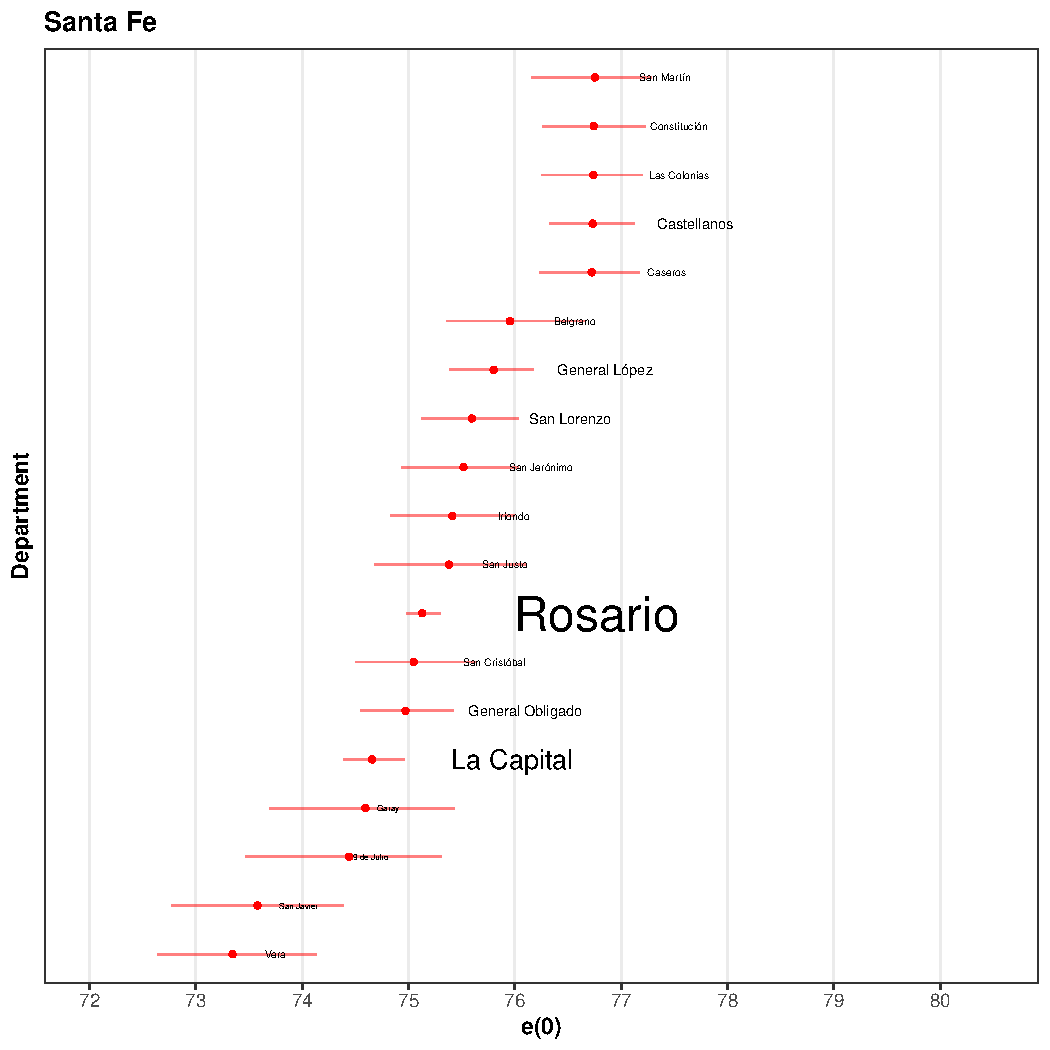
\includegraphics[width=0.6\linewidth]{C:/Proyectos/mortalidad_Argentina/analysis/plots/Santa_Fe} 

}

\end{figure}

\end{frame}

\begin{frame}

\begin{figure}

{\centering 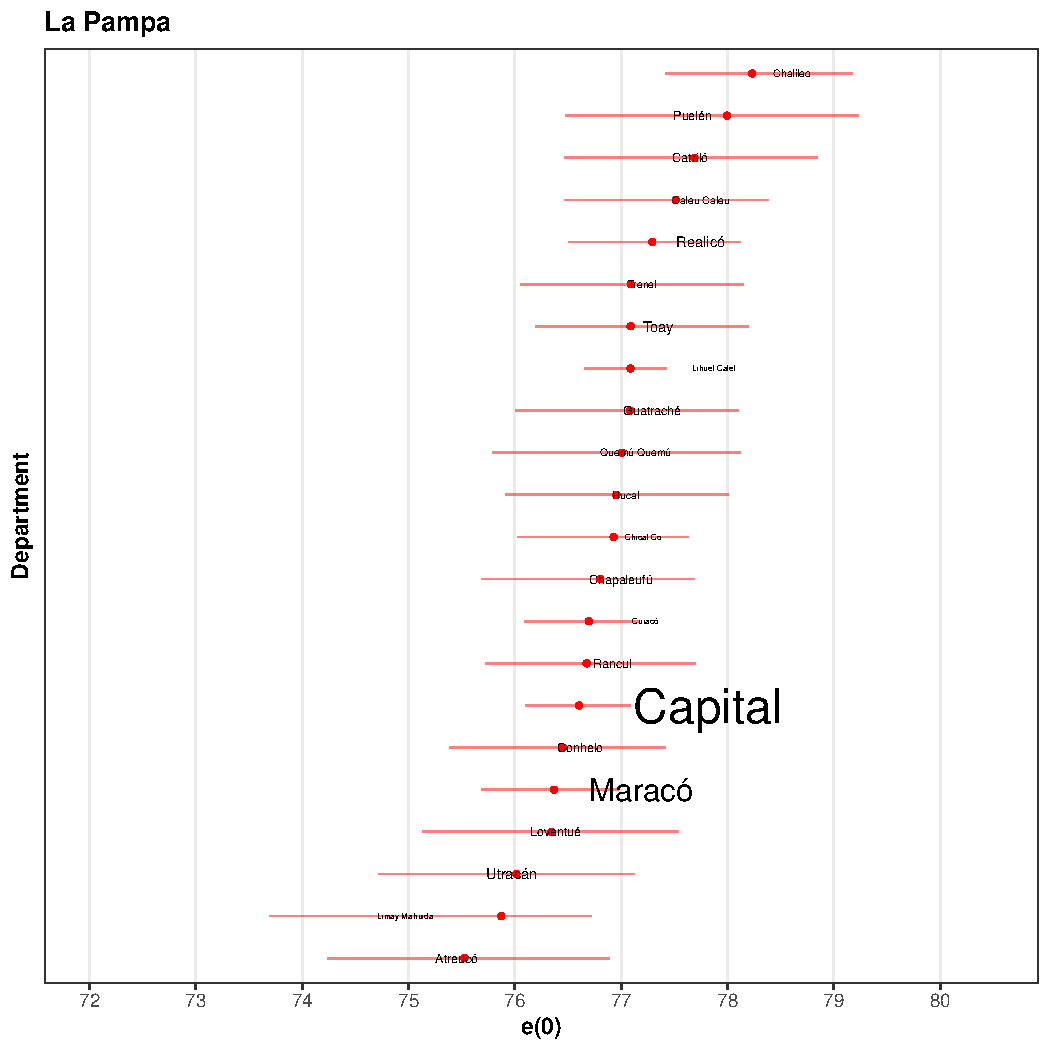
\includegraphics[width=0.6\linewidth]{C:/Proyectos/mortalidad_Argentina/analysis/plots/La_Pampa} 

}

\end{figure}

\end{frame}

\begin{frame}{Buenos Aires: 3 jurisdiccciones}

\begin{itemize}[<+->]
\tightlist
\item
  Moreno: infantil y en adultos mayores.\\
\item
  San Isidro: menor mortalidad en todas las edades.\\
\item
  Gral. Pueyrredón: 15 a 25 años.
\end{itemize}

\begin{figure}

{\centering 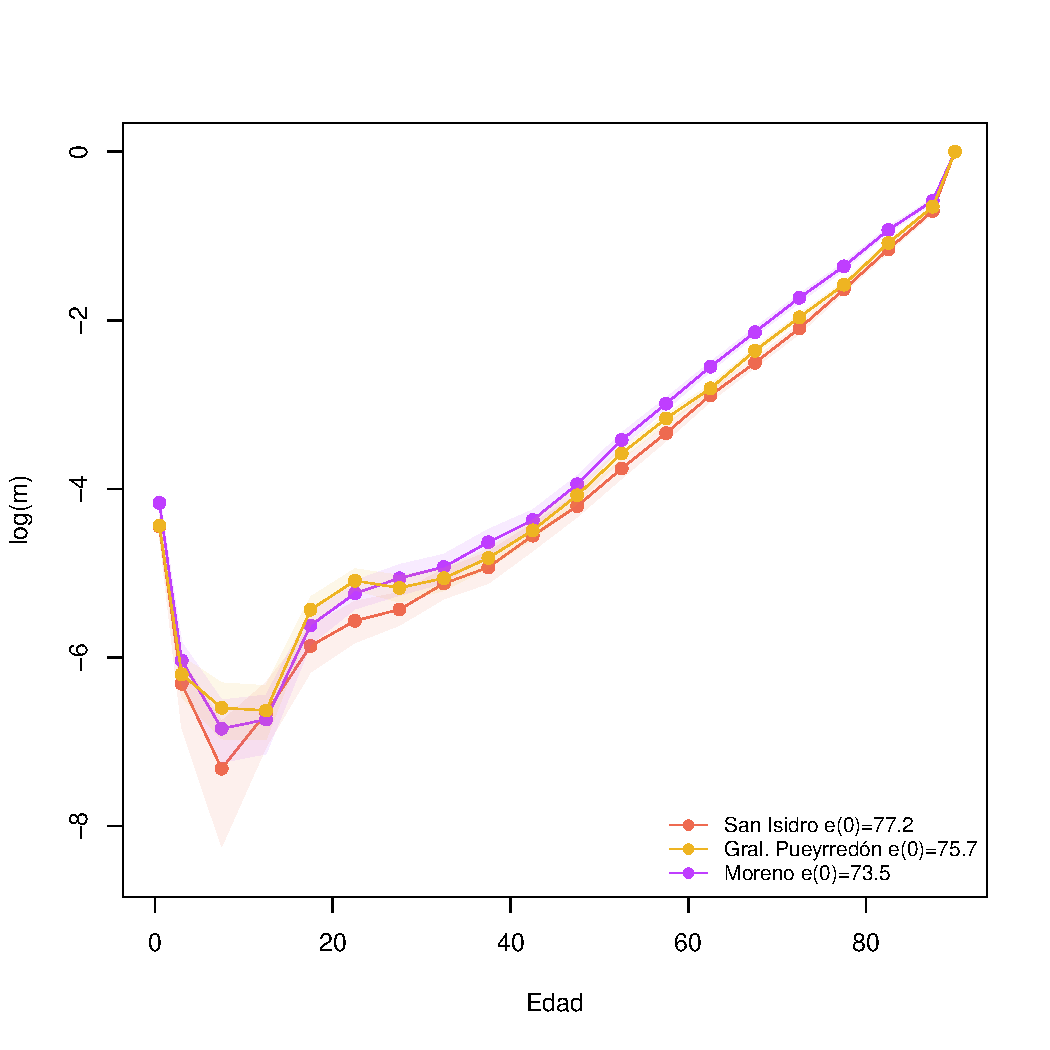
\includegraphics[width=0.65\linewidth]{C:/Proyectos/mortalidad_Argentina/analysis/plots/SanIsyMoreno} 

}

\end{figure}

\end{frame}

\begin{frame}

\begin{itemize}[<+->]
\tightlist
\item
  !Pero! ¿Qué nos permiten decir las estimaciones?
\end{itemize}

\end{frame}

\begin{frame}{Limitaciones y consideraciones}

Limitaciones:\\
* Se desconoce el nivel de cobertura de las áreas menores.\\
* Se realizaron algunas comprobaciones visuales, enfocándose
principalmente en los departamentos más poblados, pero a un
\textbf{costo} grande.

Próximos pasos:\\
+ Simular modelos de mortalidad en diferentes \textbf{escalas} y
patrones de \textbf{omisión} para la selección de la metodología.\\
+ Consistencias adicionales entre la distribución a posteriori y las
estimaciones oficiales a nivel provincial.

\end{frame}

\begin{frame}{Conclusiones}

\begin{itemize}[<+->]
\tightlist
\item
  En la búsqueda de información sobre heterogeneidad intraprovincial en
  la mortalidad
\item
  Hay decisiones en el numerador y denominador.
\item
  Se aplicaron tres métodos para estimar la estructura y el nivel de
  mortalidad, caracterizando sus diferencias principales.
\item
  Hay un \textbf{límite} en lo que podemos decir, pero podemos decir
  \textbf{algo}
\end{itemize}

\end{frame}

\section{¡Gracias!}\label{gracias}

\end{document}
